\section{Background}
\label{sec:background}

\subsection{RDMA}

\begin{figure*}[t]
    \centering
    \begin{subfigure}{0.3\linewidth}
        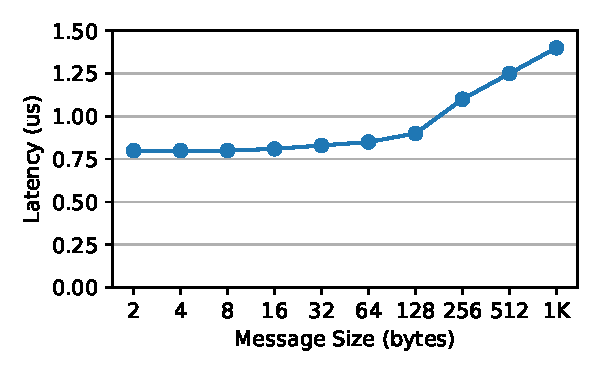
\includegraphics[width=0.99\linewidth]{fig/rdma_latency.pdf}
        \label{fig:rdma_latency}
        % \caption{}
    \end{subfigure}.
    \begin{subfigure}{0.3\linewidth}
        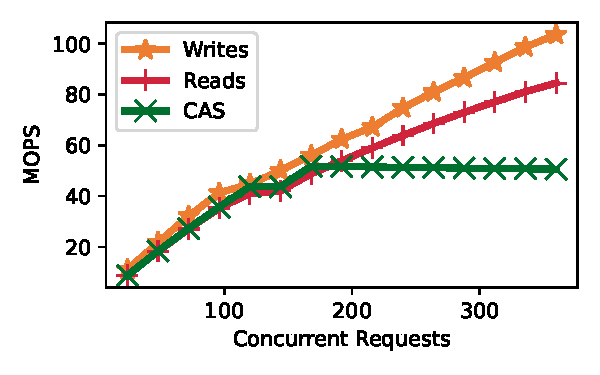
\includegraphics[width=0.99\linewidth]{fig/rdma_concur.pdf}
        % \label{fig:optimistic_failures}
        % \caption{}
    \end{subfigure}
    \begin{subfigure}{0.3\linewidth}
        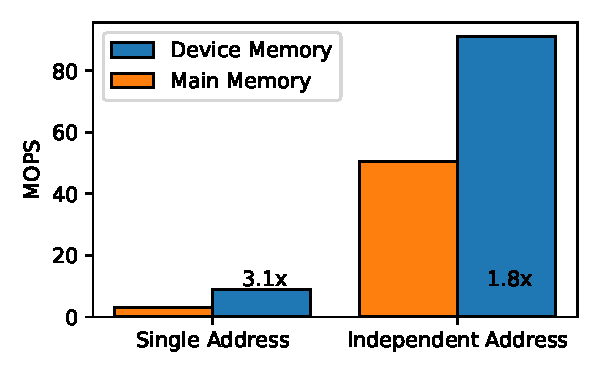
\includegraphics[width=0.99\linewidth]{fig/rdma_cas_throughput.pdf}
        % \label{fig:optimistic_failures}
        % \caption{}
    \end{subfigure}
    \vspace{-1em}
    \caption{
    \textbf{(a)} CX5 RDMA latency vs message size~\cite{rdma-latency}
    \textbf{(b)} RDMA operation scalability
    \textbf{(c)} Compare and swap performance. Device memory vs main memory.
    }
    \label{fig:rdma-benchmarks}
\end{figure*}

RDMA is an enabling technology for memory disaggregation. It
allows client machines to directly access the memory of a
remote server without the involvement of a remote CPU (save
for initialization).  Using RDMA a client can read, write, or
atomically modify remote memory using a verb api.

In the past decade the bandwidth capabilities of RDMA NICs
have increased disproportionately to their latency
improvement. The bandwidth difference between CX3 and CX7
NICs is 10$\times$ and yet intra-rack round trips of small
RDMA packets has only shrunk by around 1.5$\times$.
Comparatively bandwidth is cheaper than latency.
Figure~\ref{fig:rdma-benchmarks}(a) shows the tradeoff
between NIC to NIC round trips times on CX5 RDMA NICs for
write operations. All packets up to 128 bytes have
comparable round trip latencies, and packet sizes must grow
to above 1K before the latency cost of a large packet
exceeds the cost of two round trips for smaller packets.
\textbf{In a network with surplus bandwidth if single large
messages can be used to achieve the work of two dependent
smaller messages system latency can be improved.}

RDMA verbs do not all have the same performance. Atomic
operations such as compare-and-swap (CAS) and fetch-and-add
(FAA) both have bottlenecks much lower than reads and
writes~\cite{design-guidelines,sherman}.
Figure~\ref{fig:rdma-benchmarks}(b) shows the scalability of
these operations on CX5 NICs for 64 bit operations.
%%
Atomic operations bottleneck due to PCIe round trips. Each
operation issued from nic to host memory requires a PCIe
round trip during which time data dependent operations must
queue. Vendors have recently provided a small region (256KB)
of device mapped memory which avoids the round trip on
atomic operations~\cite{device-memory}.
Figure~\ref{fig:rdma-benchmarks}(c) shows the relative
performance of CAS operation on device memory vs host
memory. Lock request on a single address are 3x higher
throughput, and independent lock requests scale at nearly
the same rate as read and write requests.

Additionally Mellanox provides a 64-bit masked
compare-and-swap verb which allows for specific bits of a
64bit word to be set independently~\cite{rdma-masked-cas}.
This is useful for setting multiple independent locks,
assuming locks are close together, as the state of all locks
need not be known.


\subsection{RDMA Key-Value Stores}

Many projects have used RDMA to accelerate key-value
stores~\cite{farm,erpc,herd,mica,pilaf,cell,faast,storm,memc3}.
RDMA verb use is a matter of contention among these systems.
Typically reads are lock-free and made directly to remote
memory, while writes use two-sided verbs and are coordinated
by the server side CPU.
%%
Far memory key-value stores have no server side CPU and must
therefore use client side synchronization to achieve
serializablity~\cite{rolex,fusee,clover,sherman,ford,race}.
These systems make use of RDMA atomic verbs for
serialization. However, the use of the atomics is highly
dependent on the key-value stores under lying data
structure.

\textbf{Data Structures} The underlying data structures of
far-memory key value stores has a large impact on the
system's performance. To perform fast reads CPU colocated
systems have used cuckoo and hopscotch
hashing~\cite{pilaf,herd,cuckoo,hopscotch}. While these
structures have fast predictable reads, they have a large
number of updates required for insertions. These large
critical sections are amplified by far memory access times
and lead to performance bottlenecks when acquiring locks.
Recent work on remote memory data structures have opted for
optimistic concurrency~\cite{clover,race,ford,rolex,fusee}.
This strategy comes at the cost of additional round trips to
first learn up-to-date information about the remote
structure, and to ensure that the optimistic operation
completed successfully.

\textbf{Cuckoo hashing} is a hash table which delivers
constant-time reads. It uses two hash functions to determine
two possible locations at which any hashed item can reside.
When reading both locations are queried. If the item is not
found, it is not in the table. On insert, the item is placed
in the first location it hashes to. If that location is full
the item in that location is evicted and kicked to it's
second location.  This process happens iteratively for many
items. The sequence of displaced keys on an insert is called
a ~\textit{cuckoo-path}~\cite{cuckoo-improvements}. When a
loop occurs in a cuckoo path the insert fails and the table
is resized. Fill factors for cuckoo hashes can be improved
by using associative buckets for each hash index, and
shortening cuckoo paths by using BFS rather than radom
search~\cite{cuckoo-improvements}. ~\todo{consider adding a
cuckoo search figure}.